%% This is file `sample-sigconf-authordraft.tex',
%% generated with the docstrip utility.
%%
%% The original source files were:
%%
%% samples.dtx  (with options: `all,proceedings,bibtex,authordraft')
%% 
%% IMPORTANT NOTICE:
%% 
%% For the copyright see the source file.
%% 
%% Any modified versions of this file must be renamed
%% with new filenames distinct from sample-sigconf-authordraft.tex.
%% 
%% For distribution of the original source see the terms
%% for copying and modification in the file samples.dtx.
%% 
%% This generated file may be distributed as long as the
%% original source files, as listed above, are part of the
%% same distribution. (The sources need not necessarily be
%% in the same archive or directory.)
%%
%%
%% Commands for TeXCount
%TC:macro \cite [option:text,text]
%TC:macro \citep [option:text,text]
%TC:macro \citet [option:text,text]
%TC:envir table 0 1
%TC:envir table* 0 1
%TC:envir tabular [ignore] word
%TC:envir displaymath 0 word
%TC:envir math 0 word
%TC:envir comment 0 0
%%
%% The first command in your LaTeX source must be the \documentclass
%% command.
%%
%% For submission and review of your manuscript please change the
%% command to \documentclass[manuscript, screen, review]{acmart}.
%%
%% When submitting camera ready or to TAPS, please change the command
%% to \documentclass[sigconf]{acmart} or whichever template is required
%% for your publication.
%%
%%
%\documentclass[sigconf,authordraft]{acmart}
\documentclass[sigconf,review,anonymous]{acmart}
%%
%% \BibTeX command to typeset BibTeX logo in the docs
\AtBeginDocument{%
  \providecommand\BibTeX{{%
    Bib\TeX}}}

%% Rights and conference metadata are omitted for anonymous review.


%%
%% Submission ID.
%% Use this when submitting an article to a sponsored event. You'll
%% receive a unique submission ID from the organizers
%% of the event, and this ID should be used as the parameter to this command.
%%\acmSubmissionID{123-A56-BU3}

%%
%% For managing citations, it is recommended to use bibliography
%% files in BibTeX format.
%%
%% You can then either use BibTeX with the ACM-Reference-Format style,
%% or BibLaTeX with the acmnumeric or acmauthoryear sytles, that include
%% support for advanced citation of software artefact from the
%% biblatex-software package, also separately available on CTAN.
%%
%% Look at the sample-*-biblatex.tex files for templates showcasing
%% the biblatex styles.
%%

%%
%% The majority of ACM publications use numbered citations and
%% references.  The command \citestyle{authoryear} switches to the
%% "author year" style.
%%
%% If you are preparing content for an event
%% sponsored by ACM SIGGRAPH, you must use the "author year" style of
%% citations and references.
%% Uncommenting
%% the next command will enable that style.
%%\citestyle{acmauthoryear}


%%
%% end of the preamble, start of the body of the document source.
\begin{document}

%%
%% The "title" command has an optional parameter,
%% allowing the author to define a "short title" to be used in page headers.
\title{Personalizing POI Descriptions with LLMs: A Study of User Perceptions and Informational Value}

%%
%% The "author" command and its associated commands are used to define
%% the authors and their affiliations.
%% Of note is the shared affiliation of the first two authors, and the
%% "authornote" and "authornotemark" commands
%% used to denote shared contribution to the research.
\author{Anonymous Author(s)}

%%
%% By default, the full list of authors will be used in the page
%% headers. Often, this list is too long, and will overlap
%% other information printed in the page headers. This command allows
%% the author to define a more concise list
%% of authors' names for this purpose.
\renewcommand{\shortauthors}{Anonymous Author(s)}

%%
%% The abstract is a short summary of the work to be presented in the
%% article.
\begin{abstract}
Many Points of Interest (POI) descriptions remain generic and static, presenting identical content to all users regardless of interests or travel preferences. This can limit perceived relevance and may reduce engagement with travel platforms. This study examines whether large language models (LLMs) can personalize POI descriptions to improve perceived information quality. In a within-subjects study, 51 participants evaluated original and LLM-adapted descriptions across 10 POIs. Pooled rating distributions show improved perceived clarity ($p = 0.0218$, uncorrected) and borderline evidence of improved trustworthiness ($p = 0.050$), while perceived significance remained comparable ($p = 0.30$). Optional post-study responses indicate relatively high comfort with AI-generated travel content (mean = 3.94, $n = 17$). These findings suggest that LLM-based personalization can improve perceived clarity in tourism micro-content without clear losses in perceived credibility.
\end{abstract}

%%
%% The code below is generated by the tool at http://dl.acm.org/ccs.cfm.
%% Please copy and paste the code instead of the example below.
%%
\begin{CCSXML}
<ccs2012>
   <concept>
	<concept_id>10003120.10003121.10003122.10003334</concept_id>
	<concept_desc>Human-centered computing~User studies</concept_desc>
	<concept_significance>300</concept_significance>
	</concept>
	<concept>
	<concept_id>10003120.10003123.10010860.10010859</concept_id>
	<concept_desc>Human-centered computing~User centered design</concept_desc>
	<concept_significance>500</concept_significance>
	</concept>
 </ccs2012>
\end{CCSXML}

\ccsdesc[500]{Human-centered computing~User centered design}
\ccsdesc[300]{Human-centered computing~User studies}

%%
%% Keywords. The author(s) should pick words that accurately describe
%% the work being presented. Separate the keywords with commas.
\keywords{poi adaptation, LLM-generated content, ai-driven descriptions, content personalization}
%% A "teaser" image appears between the author and affiliation
%% information and the body of the document, and typically spans the
%% page.
%\begin{teaserfigure}
 % 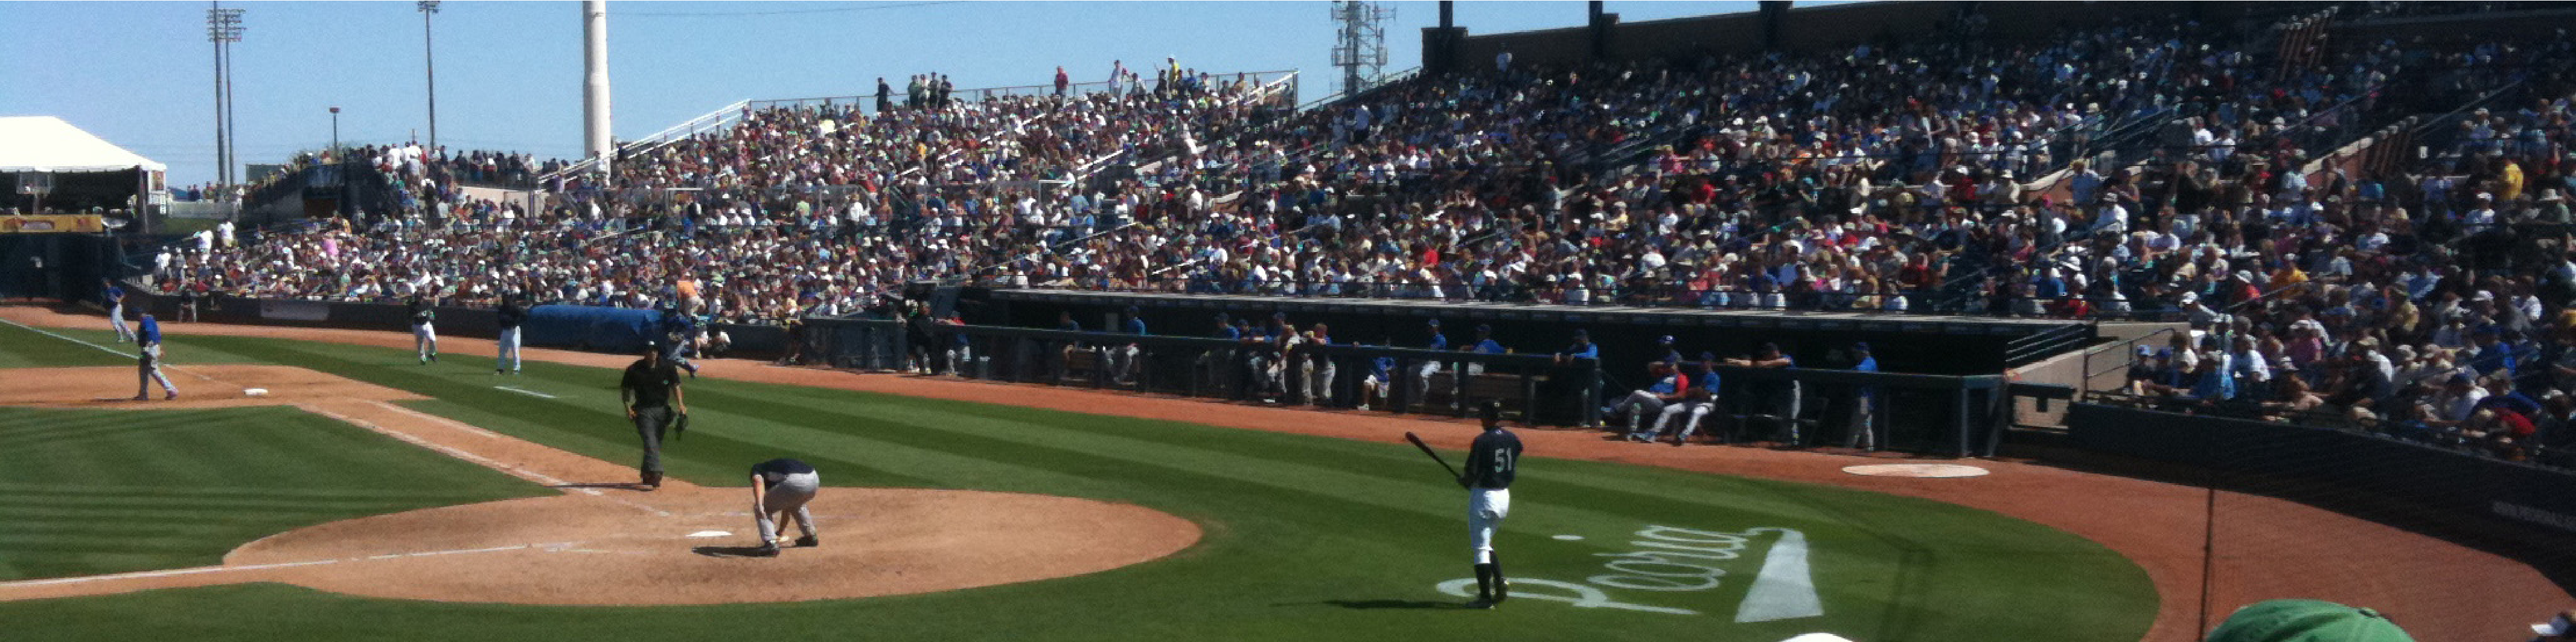
\includegraphics[width=\textwidth]{sampleteaser}
  %\caption{Seattle Mariners at Spring Training, 2010.}
  %\Description{Enjoying the baseball game from the third-base
  %seats. Ichiro Suzuki preparing to bat.}
  %\label{fig:teaser}
%\end{teaserfigure}

%% Submission and acceptance metadata are omitted for anonymous review.

%%
%% This command processes the author and affiliation and title
%% information and builds the first part of the formatted document.
\maketitle

\section{Introduction}
Personalization has become a key factor in improving user engagement in various digital experiences, including travel and tourism. As travellers seek more relevant and tailored recommendations, AI advancements, particularly large language models (LLM), presents new opportunities to adapt content to align with individual preferences dynamically. One such application is personalized descriptions of Points of Interest (POIs), such as hotels, restaurants, museums, and gardens. Although traditional POI descriptions are often static and generalized, AI-driven personalization can refine these descriptions to match user-specific interests, past experiences, and contextual relevance, enhancing both engagement and comprehension.

Much prior research has focused on POI recommendation and ranking systems, where AI models suggest locations based on user preferences, behaviors, and contextual factors. However, less attention has been given to how the content of each POI itself can be adapted to better engage users. When individuals access POI descriptions, the same information is typically presented to all users, despite variations in their backgrounds, interests, and motivations to visit a place. For example, a museum description could emphasize historical significance for a history enthusiast while focusing on interactive exhibits for a family traveler. Generative AI and LLMs provide a unique opportunity to dynamically tailor content without altering its factual meaning, ensuring that the description remains relevant and appealing to different audiences.

To explore this potential, a prototype system was developed that allows users to enter their preferences and interests and then dynamically presents two versions of each POI description: the original and an LLM-adapted version. Participants were asked to evaluate the descriptions based on alignment with their preferences, perceived appeal, and familiarity with the location. The key objective is to assess whether AI-generated adaptations are acceptable and meaningful, effectively convey the original value of POI, and improve user engagement.

This study contributes to the growing field of AI-powered content personalization in tourism by investigating the role of LLMs in dynamic adaptation of textual content. By analyzing participant feedback, this study aims to provide insight into how AI-generated descriptions can improve engagement while preserving accuracy and authenticity.

% The remainder of this paper is structured as follows. Section 2 details the methodology, including the experimental setup, data collection process, and evaluation metrics. Section 3 presents the results and analysis of user perceptions across significance, trustworthiness, and clarity dimensions. Section 4 discusses the implications of the findings and limitations of the study. Section 5 outlines directions for future research, and Section 6 concludes with key takeaways and practical implications for tourism platforms.


\section{Related work}

Prior work on tourism and location-based personalization has largely focused on point-of-interest (POI) recommendation, where systems predict or rank places that match a user profile and context. Surveys of travel and POI recommenders highlight the importance of heterogeneous signals such as mobility patterns, time, geography, and user attributes, as well as evaluation challenges that arise from contextual variability and data sparsity \cite{renjith_extensive_2020,wang_survey_2025}. Recent work in the UMAP community also emphasizes that user preferences can differ before and after a visit, which complicates modeling and suggests that preference signals and content expectations are not static \cite{hofschen_expected_2023}.

With the rise of large language models (LLMs), research has expanded to interactive and generative paradigms for personalization, including LLM-based pipelines for POI recommendation and user profile generation \cite{wang_embracing_2024,wang_point--interest_2025,Li2024SIGIR_LLMNextPOI,noauthor_genup_nodate}. Tourism research has also begun evaluating generative AI for content creation and trip planning \cite{li_generative_2025,zhang_co-creating_2024,hsu_fine-tuned_2024}. However, these works often study destination promotion or end-to-end planning rather than the micro-content users read when deciding whether a POI is relevant. This study addresses this gap by adapting POI descriptions to user interest profiles while keeping core facts stable, measuring perceptions of significance, trustworthiness, and clarity.



\section{Methodology}
%This section outlines the methodology employed to evaluate the effectiveness of LLM-generated personalized POI descriptions compared to original manual descriptions. The study design, description personalization process, evaluation interface, metrics, procedure, and participant recruitment are described below.
This study examines how users perceive LLM-adapted POI descriptions in comparison to original, manually written descriptions. It focuses on perceived information quality, specifically clarity, trustworthiness, and relevance, rather than on recommendation accuracy or task performance. We conducted a user-centered comparative study in which participants evaluated paired descriptions of the same POI. Each pair included an original description sourced from existing online material and an LLM-adapted version personalized using the participant’s stated preferences. Participants were not informed which description was AI-generated, ensuring that evaluations reflected perceived qualities rather than source awareness.

\subsection{Study Design}
A within-subjects experimental design was employed in which each participant evaluated both original and AI-personalized descriptions for multiple POIs. This design enabled direct comparison between description types while controlling for individual differences in preferences and expectations. The study presented participants with 10 POIs spanning five categories (two per category): accommodation (Hotel Hassler Roma, The Savoy), natural attractions (Jungfraujoch, Neuschwanstein Castle), entertainment (Cologne Carnival, Cannstatter Volksfest), cultural and historical sites (Colosseum, Louvre Museum), and commercial destinations (Via del Corso, Caf\'{e} Central Vienna). POIs were selected to include both internationally recognized locations (e.g., Colosseum, Louvre) and regionally significant destinations (e.g., Cannstatter Volksfest), providing variety in familiarity levels.

\subsection{Participants}
A total of 51 participants were recruited through personal networks via email and direct messaging. Participants were required to be at least 18 years old and possess basic English proficiency to ensure effective engagement with POI descriptions. No specific travel experience was mandated, as the study aimed to assess AI-generated descriptions across diverse user segments.

Participants ranged from 22 to 49 years old ($\mu = 30.94$, $\sigma = 6.74$), with 67\% male and 33\% female. The sample was predominantly Indian (n = 28) and German (n = 21), with additional participants from China (n = 1) and Iran (n = 1). Professionally, participants included students (n = 22), engineers (n = 16), academics (n = 3), and other professions (n = 10). Most reported intermediate (n = 21) or experienced (n = 19) travel levels. The sample's geographic concentration reflects convenience sampling through personal networks rather than stratified recruitment; accordingly, findings should be interpreted as applicable to technology-familiar, educated populations with similar demographics.

\subsection{LLM-Based Personalization of POI Descriptions}
To operationalize personalization in the study, we employed a lightweight and explicit user profile derived from participants’ self-reported attributes and preferences. The profile was not intended as a predictive user model, but rather as a structured representation of personal context used to guide content adaptation. Personalization focused on adjusting emphasis and framing within POI descriptions while preserving their original meaning and factual content.

For each POI, two description versions were prepared. The original description was sourced from official tourism websites and travel platforms, representing standard, non-personalized content. The AI-adapted version was generated using gpt-4o-2024-11-20\footnote{\url{https://platform.openai.com/docs/models/gpt-4o}} with the default temperature setting. The model received a system prompt instructing it to act as an expert travel writer, emphasizing unique aspects, cultural significance, and visitor experience while adapting content to the user's situation. The user prompt included ten personalization dimensions: age, gender, marital status, whether the user has children, interests, travel experience level, education, profession, hobbies, and preferred travel style. The original POI title and description were provided, and the model was instructed to maintain factual accuracy and length, while emphasizing aspects most relevant to the user's profile. To verify factual preservation, a subset of generated descriptions was manually reviewed during initial testing to confirm that no factual claims were altered or fabricated during personalization. For example, a museum description for a participant interested in history would emphasize historical significance and artifacts, while the same museum described for a family traveler would highlight interactive exhibits and educational programs.

\subsection{Evaluation Interface}
Participants viewed descriptions through a web-based interface that displayed two versions side by side, labeled as Version A and Version B (see Figure~\ref{fig:eval-interface}). The interface did not indicate which version was AI-generated. Each POI was accompanied by a representative image to provide visual context. The presentation order of AI and manual descriptions was randomized across POIs to prevent order bias. Participants could not proceed to the next POI without completing evaluations for the current one, ensuring complete data collection.

\begin{figure*}[h]
  \centering
  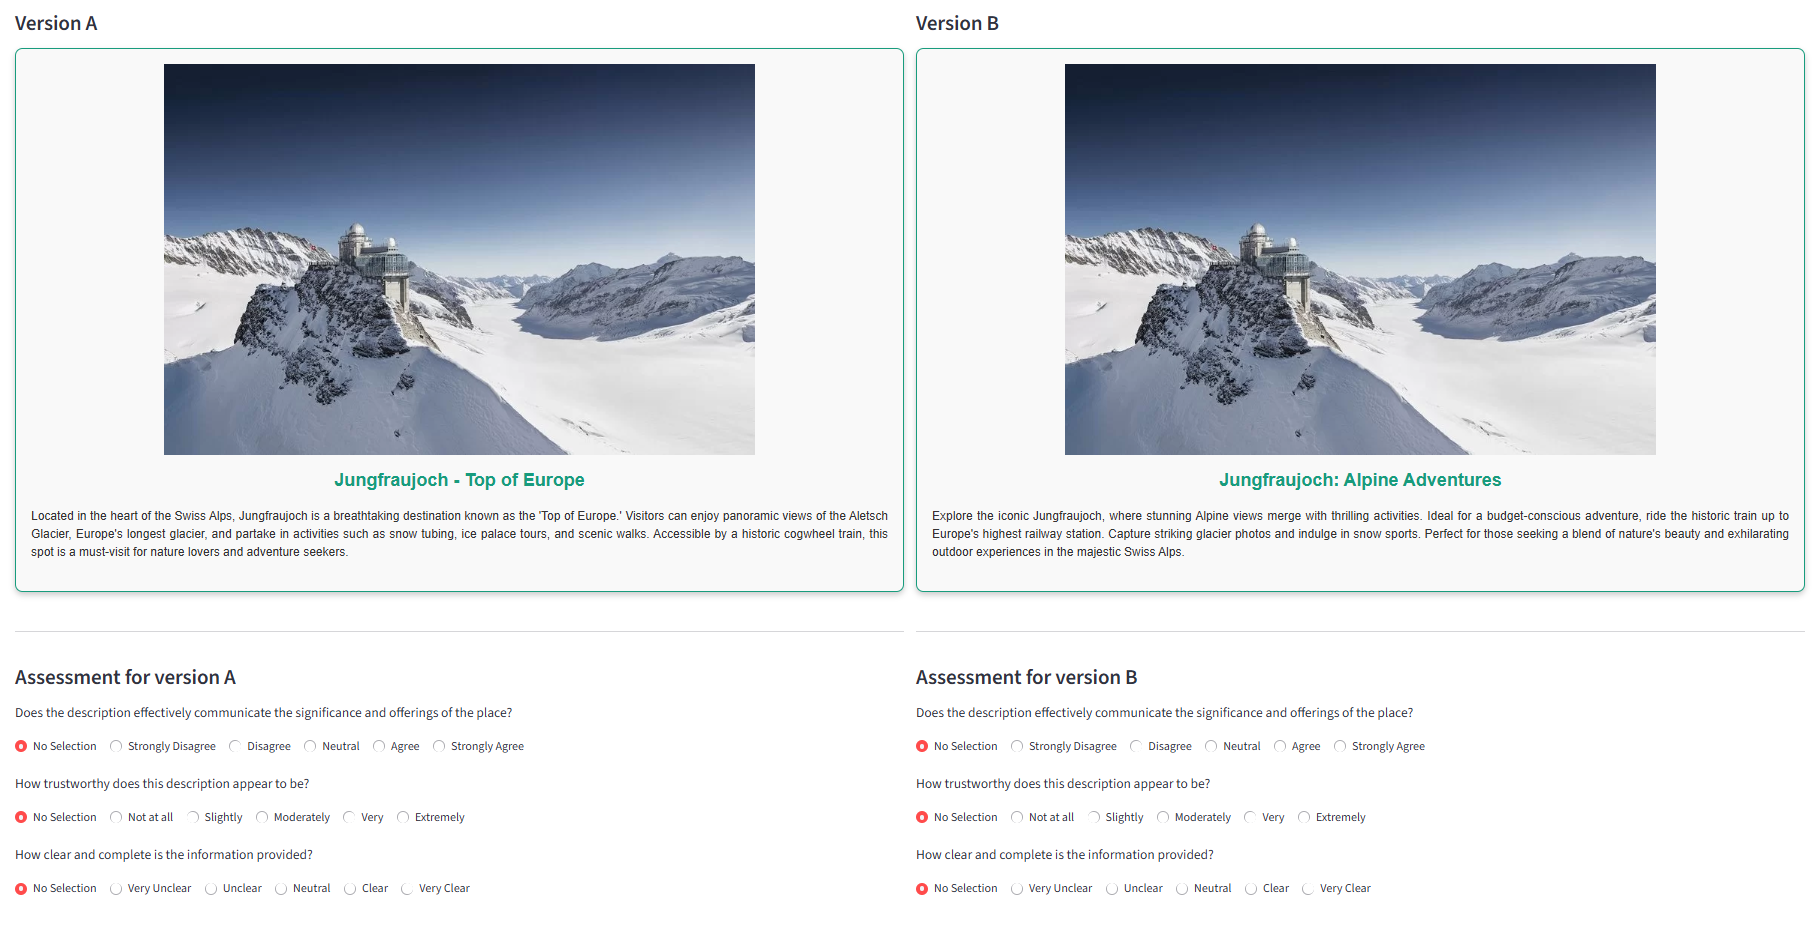
\includegraphics[width=0.90\linewidth]{figures/PoI_survey_img.png}
  \caption{Evaluation interface showing two description versions (Version A and Version B) presented side by side for participant comparison}
  \Description{Screenshot of the evaluation interface displaying two POI description versions with an image of Jungfraujoch mountain peak}
  \label{fig:eval-interface}
\end{figure*}

\subsection{Information Quality Measures}

Participants assessed each POI description along three perceptual dimensions using 5-point scales:
\begin{itemize}
    \item \textbf{Significance}: ``Does the description effectively communicate the significance and offerings of the place?'' (5-point agreement scale: 1 = Strongly Disagree, 5 = Strongly Agree)
    \item \textbf{Trustworthiness}: ``How trustworthy does this description appear to be?'' (5-point intensity scale: 1 = Not at all, 5 = Extremely)
    \item \textbf{Clarity}: ``How clear and complete is the information provided?'' (5-point clarity scale: 1 = Very Unclear, 5 = Very Clear)
\end{itemize}

After rating both descriptions individually, participants completed comparative judgments indicating which description was more engaging, informative, appealing, and more likely to encourage a visit. Participants also reported their prior familiarity with each POI (visited, heard of, or unfamiliar).


%\subsection{Statistical Analysis}
%Results are summarized using mean ratings across all POIs and participants ($N = 510$ paired observations per metric). Because each participant evaluated both manual and AI-adapted descriptions for the same POI, paired statistical tests were employed to account for the within-subjects design. Specifically, paired $t$-tests assessed mean differences under the assumption of normally distributed difference scores, while Wilcoxon signed-rank tests provided a non-parametric alternative that does not assume normality. Both tests were applied to each metric (significance, trustworthiness, and clarity) to ensure robustness of conclusions. Statistical significance was evaluated at $\alpha = 0.05$.

\subsection{Procedure}
The study was conducted in three phases using a secure web platform.  First, participants reviewed an informed consent form explaining the study purpose, voluntary participation, and data confidentiality. After providing consent, they completed a demographic and preference survey collecting age, gender, nationality, profession, current city, hobbies, preferred travel styles, and tourism interests. This information formed the basis for personalizing AI-generated descriptions. The interface required a minimum number of preference selections to ensure sufficiently expressive profiles. Based on this information, POI descriptions were automatically generated using a large language model in subsequent pages of the study.

Participants then proceeded to the main evaluation phase, where they were presented with POI descriptions adapted using their profile information alongside original descriptions. The adapted descriptions were generated dynamically after the profiling step and before the evaluation, without further user interaction. Second, participants evaluated 10 POIs sequentially by reading both description versions and rating them on core metrics and familiarity. This evaluation phase lasted approximately 20 to 30 minutes. Finally, participants provided overall feedback on their experience and their comfort level with AI-generated travel content. All data were collected anonymously to ensure privacy. The study was conducted in accordance with institutional ethical guidelines, with participants providing informed consent before participation.
% The study proceeded in three phases. First, participants reviewed an informed consent form explaining the study purpose, voluntary participation, and data confidentiality. After providing consent, they completed a demographic and preference survey collecting age, gender, nationality, profession, current city, hobbies, preferred travel styles, and tourism interests. This information formed the basis for personalizing AI-generated descriptions.

% Second, participants entered the main evaluation phase, viewing 10 POIs sequentially. For each POI, they read both description versions, rated each individually on the three core metrics, completed comparative evaluations, and indicated their familiarity with the location. The entire evaluation phase took approximately 20 to 30 minutes.

% Third, upon completing all POI evaluations, participants provided overall feedback rating their experience with the study, their opinion on automated description adaptation, and their comfort level with AI-generated travel content. All responses were collected anonymously through a secure web platform, ensuring participant privacy and compliance with ethical research standards.




\section{Results}
This section presents findings from the user study evaluating LLM-adapted POI descriptions against manual baselines. Responses are summarized across three core metrics: significance, trustworthiness, and clarity. Comparative preference results and overall feedback are then reported.

Across 51 participants and 10 POIs, the study collected $N = 510$ ratings per condition for each metric (manual versus AI). Table~\ref{tab:metrics-summary} summarizes the distribution of ratings aggregated across all evaluations.

\begin{table}[h]
  \centering
  \small
  \begin{tabular}{@{}lcccccc@{}}
    \toprule
    & \multicolumn{2}{c}{\textbf{Significance}} & \multicolumn{2}{c}{\textbf{Trust}} & \multicolumn{2}{c}{\textbf{Clarity}} \\
    \cmidrule(lr){2-3} \cmidrule(lr){4-5} \cmidrule(lr){6-7}
    \textbf{Level} & Man. & AI & Man. & AI & Man. & AI \\
    \midrule
    1--2 (Low)  & 5.5  & 6.3  & 10.0 & 7.3  & 7.1  & 5.7 \\
    3 (Neutral) & 27.1 & 23.1 & 33.3 & 27.4 & 28.8 & 21.4 \\
    4--5 (High) & 67.4 & 70.6 & 56.7 & 65.3 & 64.1 & 72.9 \\
    \bottomrule
  \end{tabular}
  \vspace{0.9em}
  \caption{Distribution of User Ratings (\%) for Manual vs.\ AI Descriptions ($N=510$)}
  \label{tab:metrics-summary}
\end{table}

% Full count tables are available in the accompanying research report.

\subsection{Perceived Significance}
Participants rated both description versions on how effectively they communicated the significance and offerings of each POI using a 5-point Likert scale ranging from Strongly Disagree to Strongly Agree. Figure~\ref{fig:significance} illustrates the distribution of responses for manual and AI-generated descriptions.

\begin{figure}[h]
  \centering
  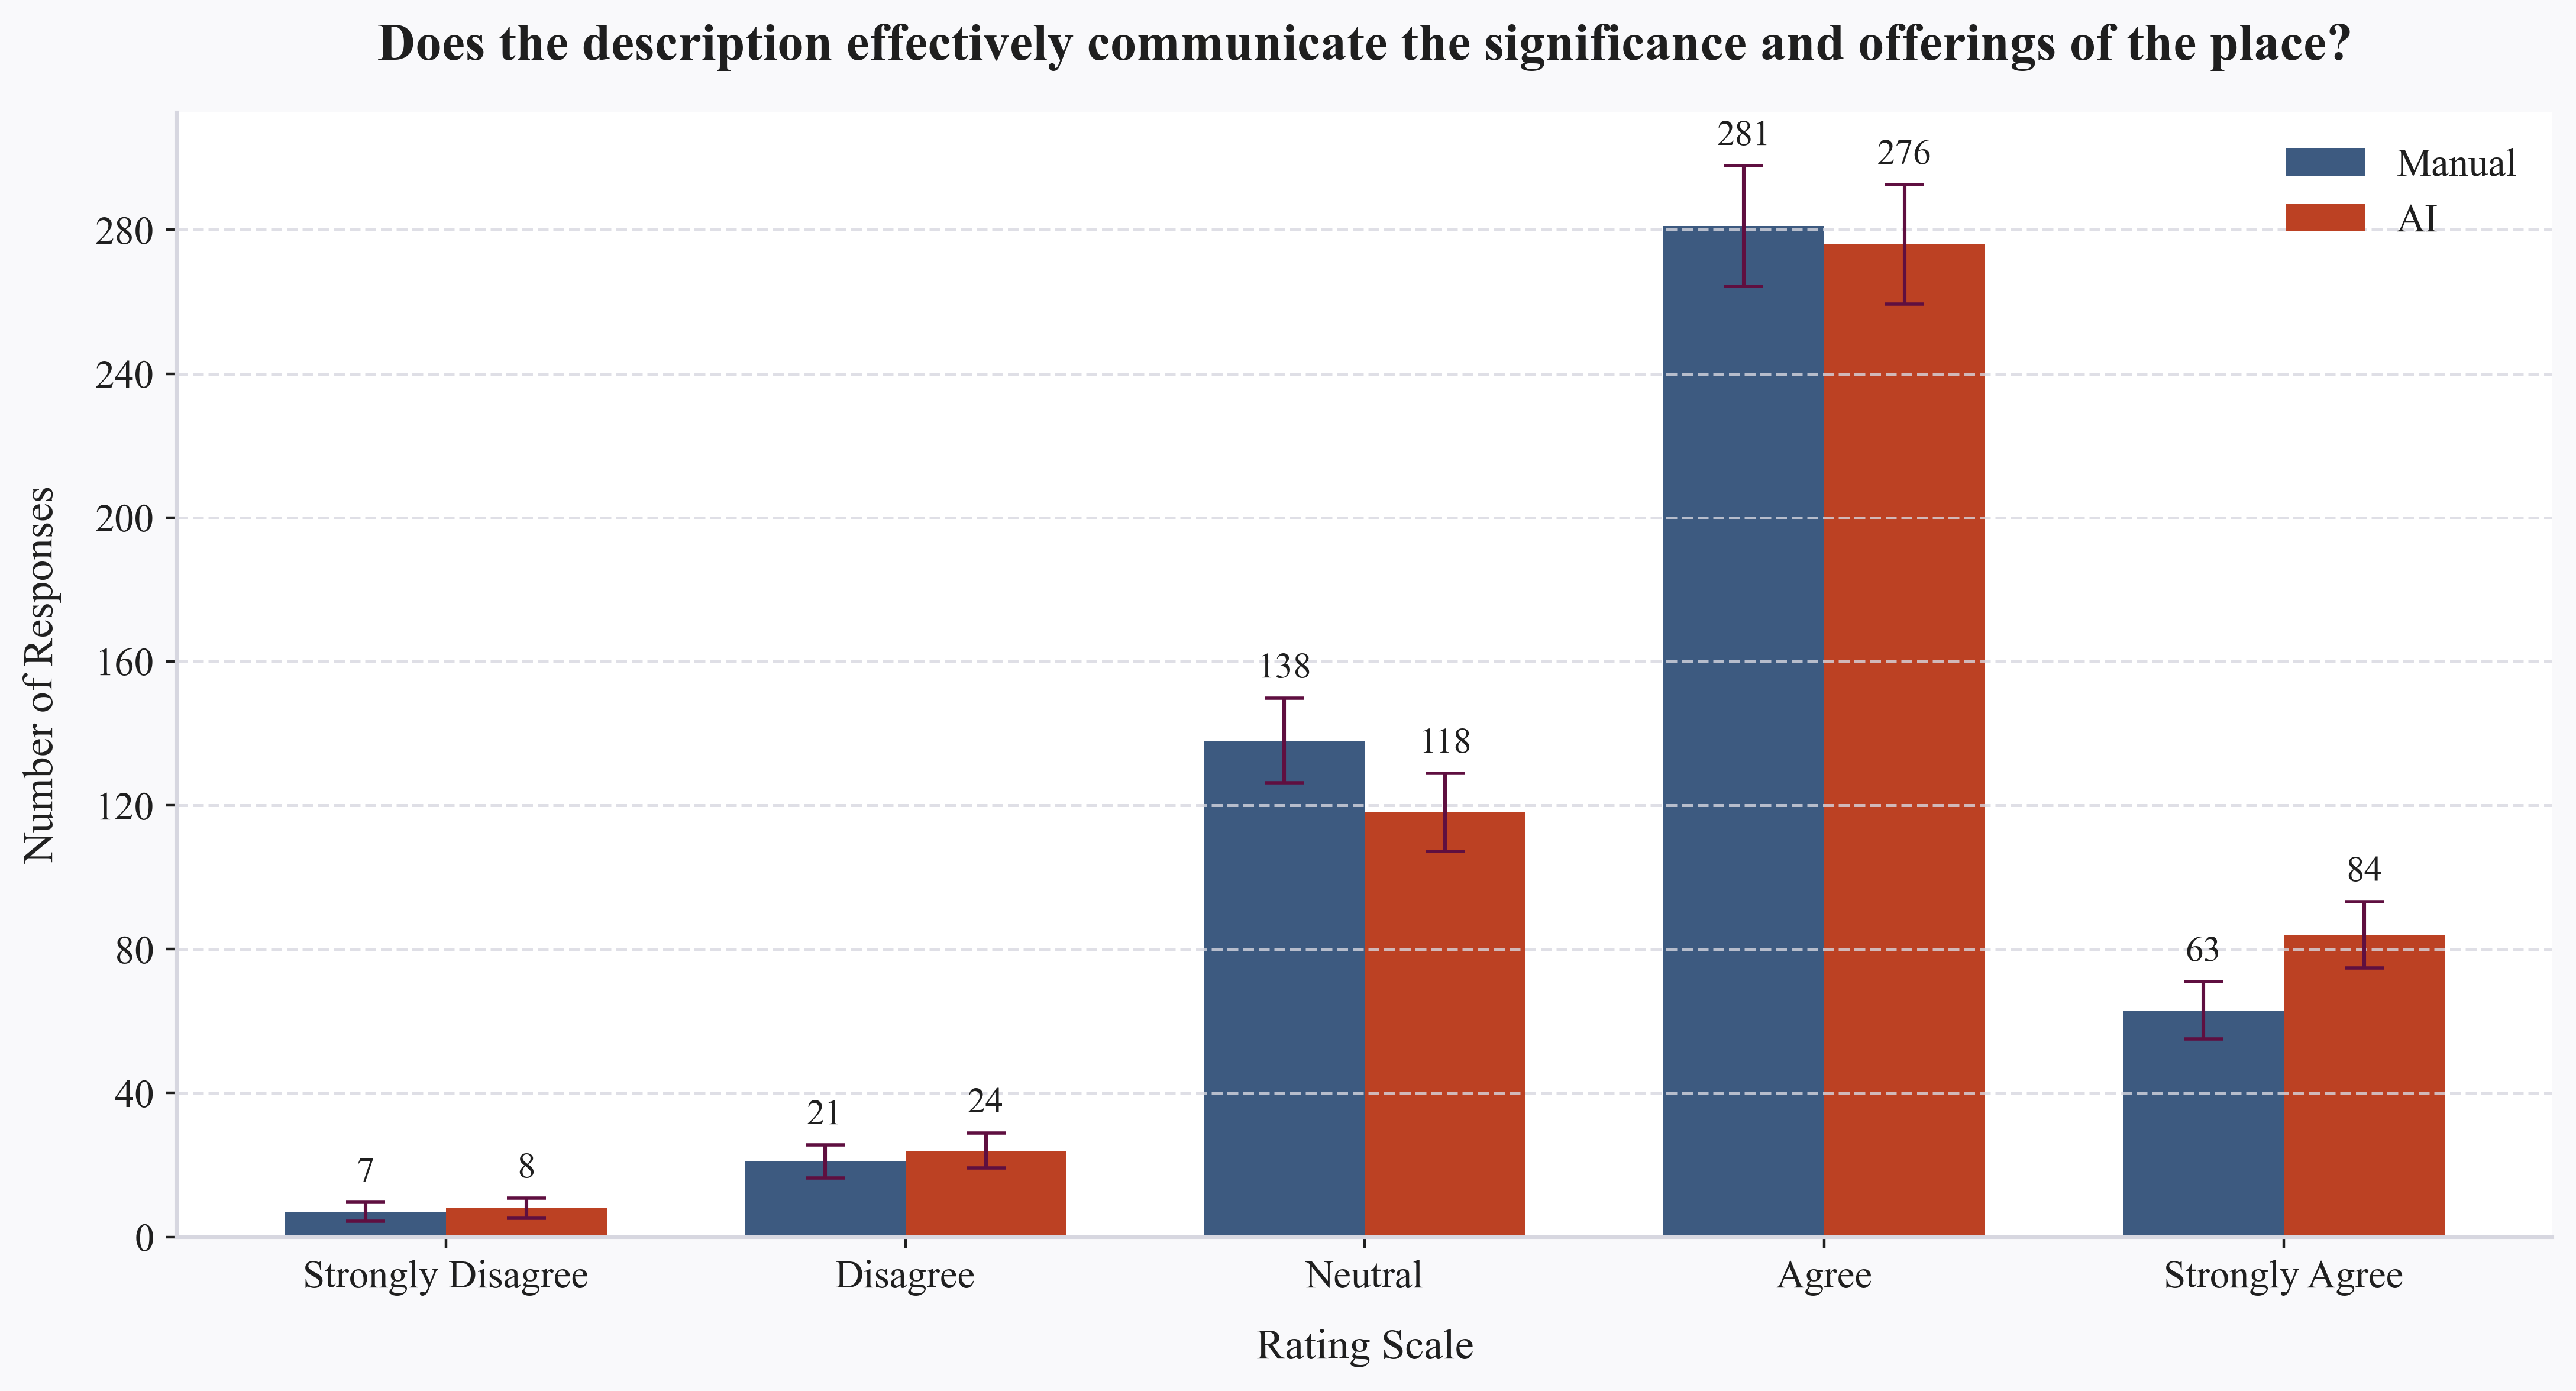
\includegraphics[width=0.85\linewidth]{figures/significance_comparison.png}
  \caption{Comparison of perceived significance between manual and AI-generated descriptions. Error bars represent Poisson-style standard error estimates computed on raw counts ($\sqrt{n}$).}
  \Description{Bar chart comparing manual and AI description ratings for significance communication}
  \label{fig:significance}
\end{figure}

Both description types received predominantly positive ratings (Table~\ref{tab:metrics-summary}). AI-generated descriptions shifted responses away from neutral toward stronger endorsement (e.g., Strongly Agree increased from 63 to 84 ratings). However, the pooled chi-square test did not indicate a statistically reliable difference in the overall distribution ($\chi^2(4) = 4.87$, $p = 0.3005$). The corresponding effect size was small (Cramer's $V = 0.069$, computed with $N=1020$ pooled observations), suggesting similar perceived significance between conditions.

\subsection{Trustworthiness}
Trustworthiness was assessed on a 5-point scale ranging from Not at all to Extremely. Figure~\ref{fig:trust} presents the comparative distribution of trust ratings.

\begin{figure}[h]
  \centering
  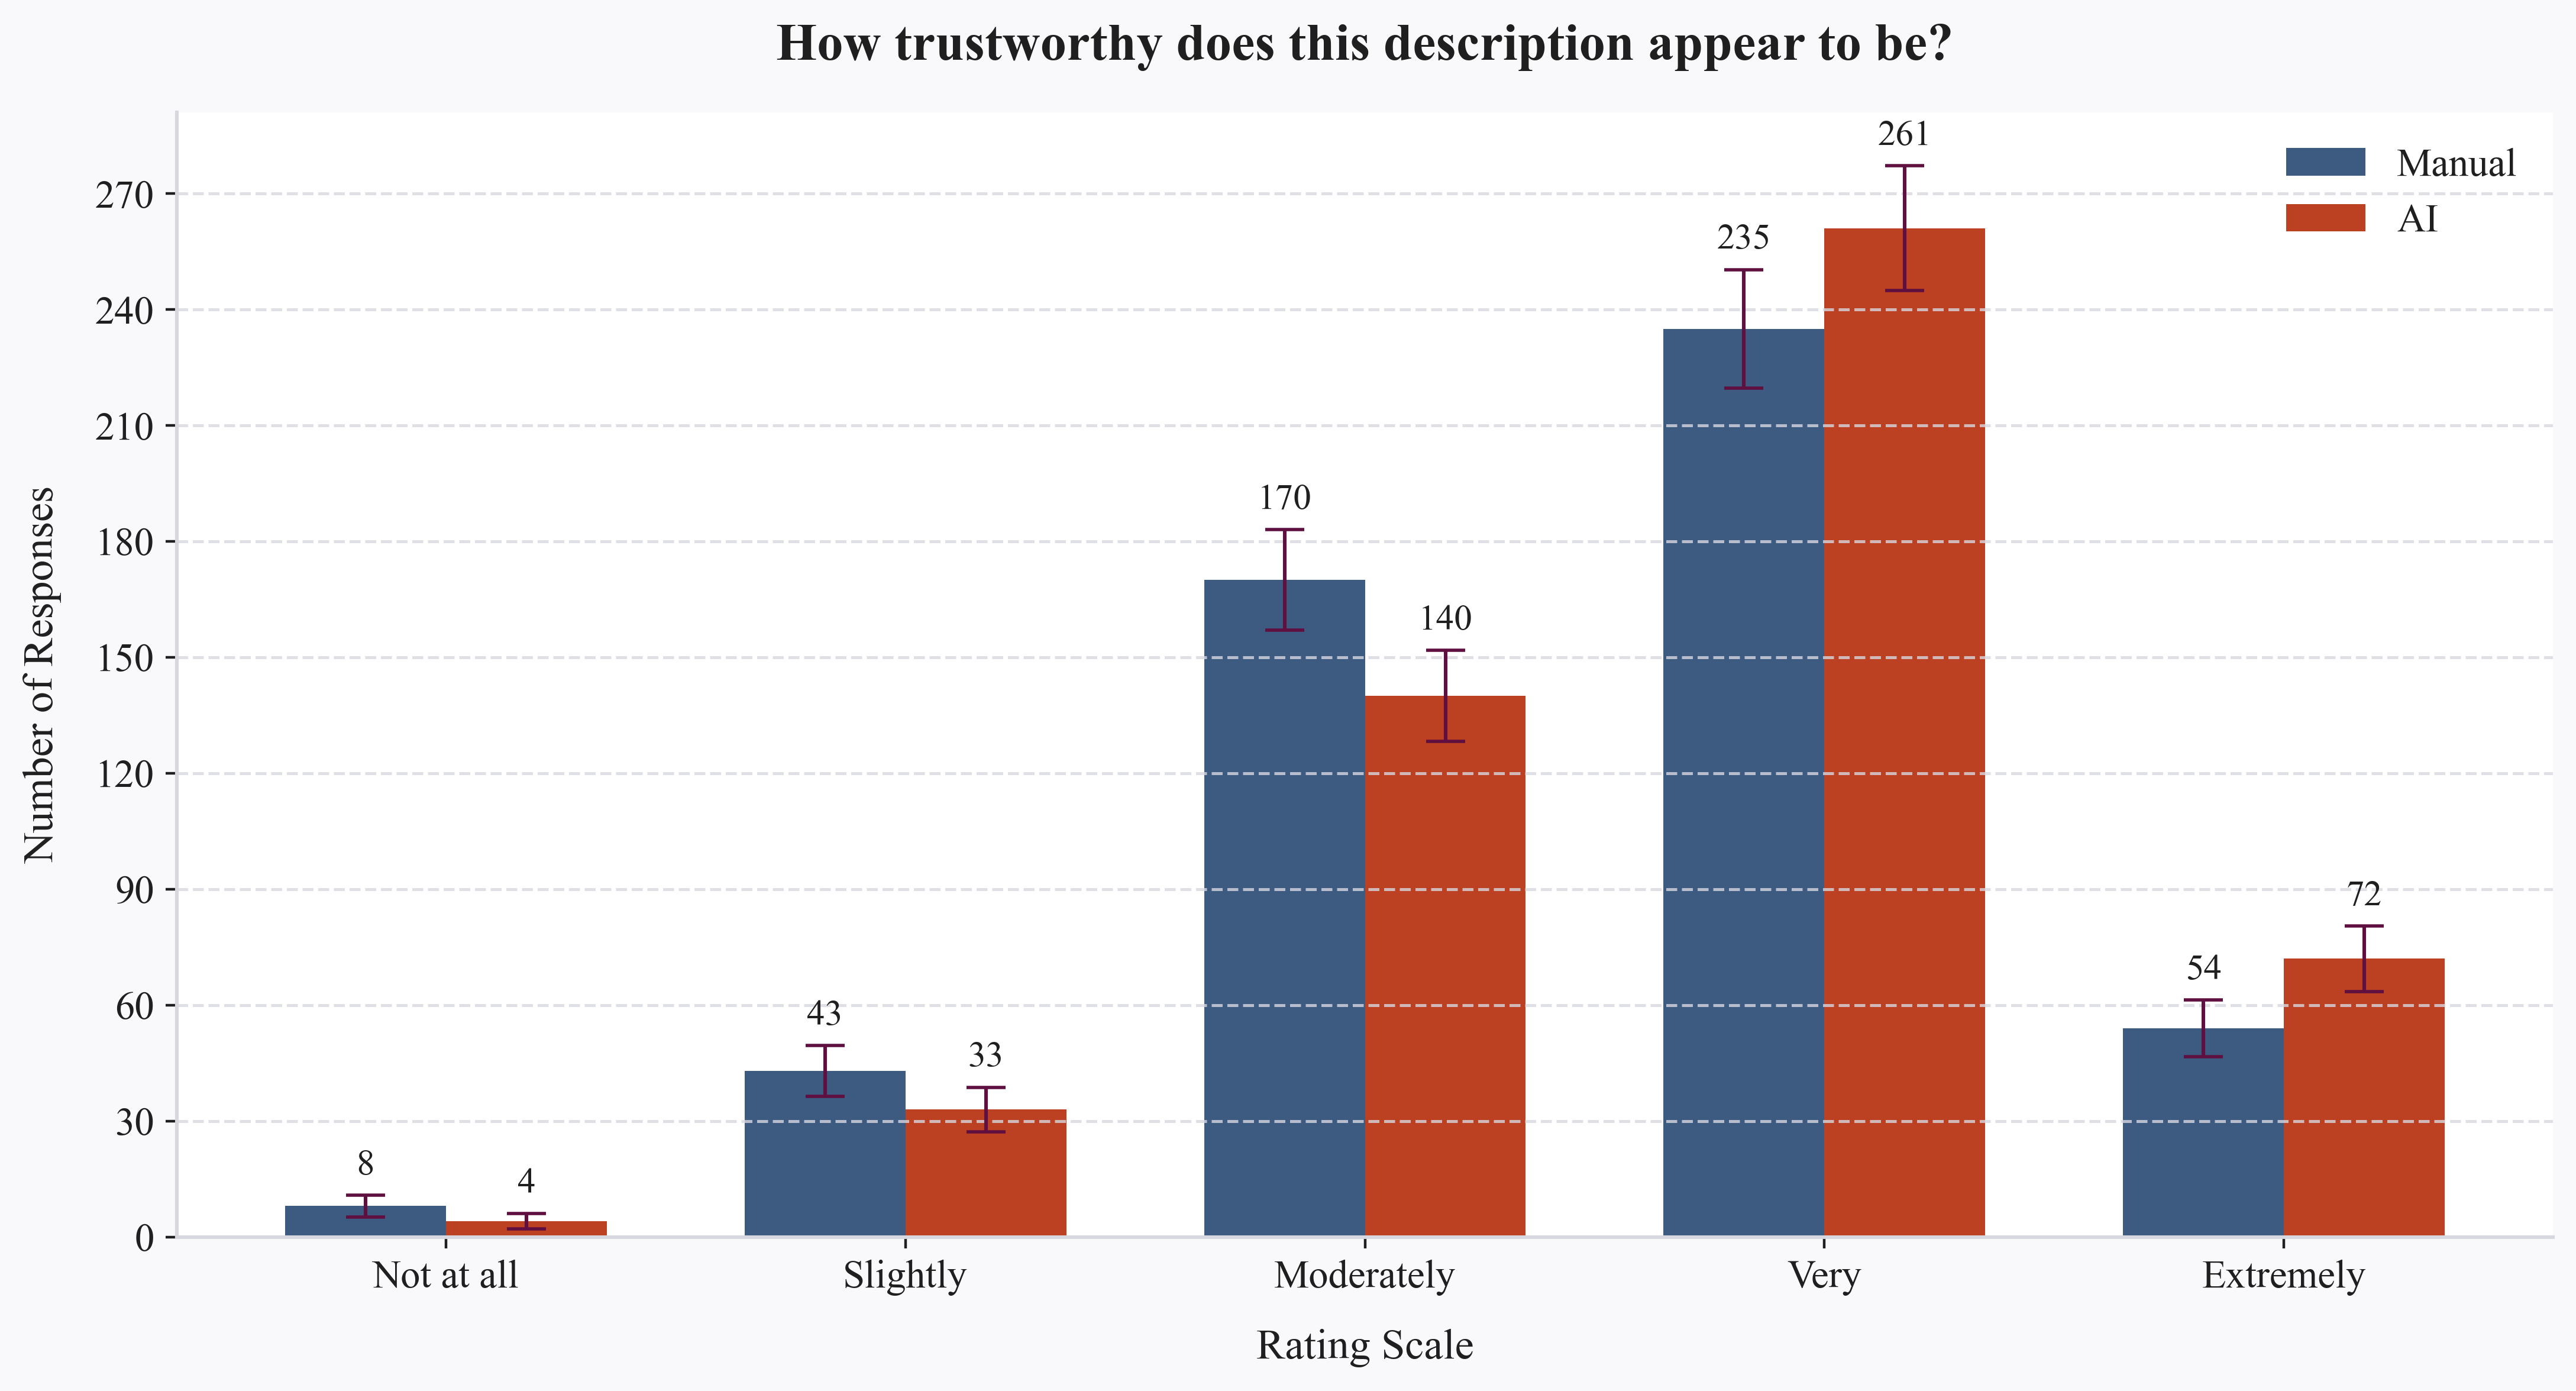
\includegraphics[width=0.85\linewidth]{figures/trust_comparison.png}
  \caption{Comparison of perceived trustworthiness between manual and AI-generated descriptions. Error bars represent Poisson-style standard error estimates computed on raw counts ($\sqrt{n}$).}
  \Description{Bar chart comparing manual and AI description ratings for trustworthiness}
  \label{fig:trust}
\end{figure}

AI-generated descriptions received higher trust ratings overall, with fewer low-trust responses and more ratings in the highest category (Extremely: 72 vs.
54). The pooled chi-square test provided borderline evidence of a distributional shift ($\chi^2(4) = 9.49$, $p = 0.050$). The effect size was small (Cramer's $V = 0.096$, computed with $N=1020$ pooled observations), indicating that the improvement is modest in magnitude and should be interpreted cautiously.

\subsection{Clarity and Completeness}
Participants evaluated how clear and complete the information was using a 5-point scale from Very Unclear to Very Clear. Figure~\ref{fig:clarity} shows the distribution of clarity ratings.

\begin{figure}[h]
  \centering
  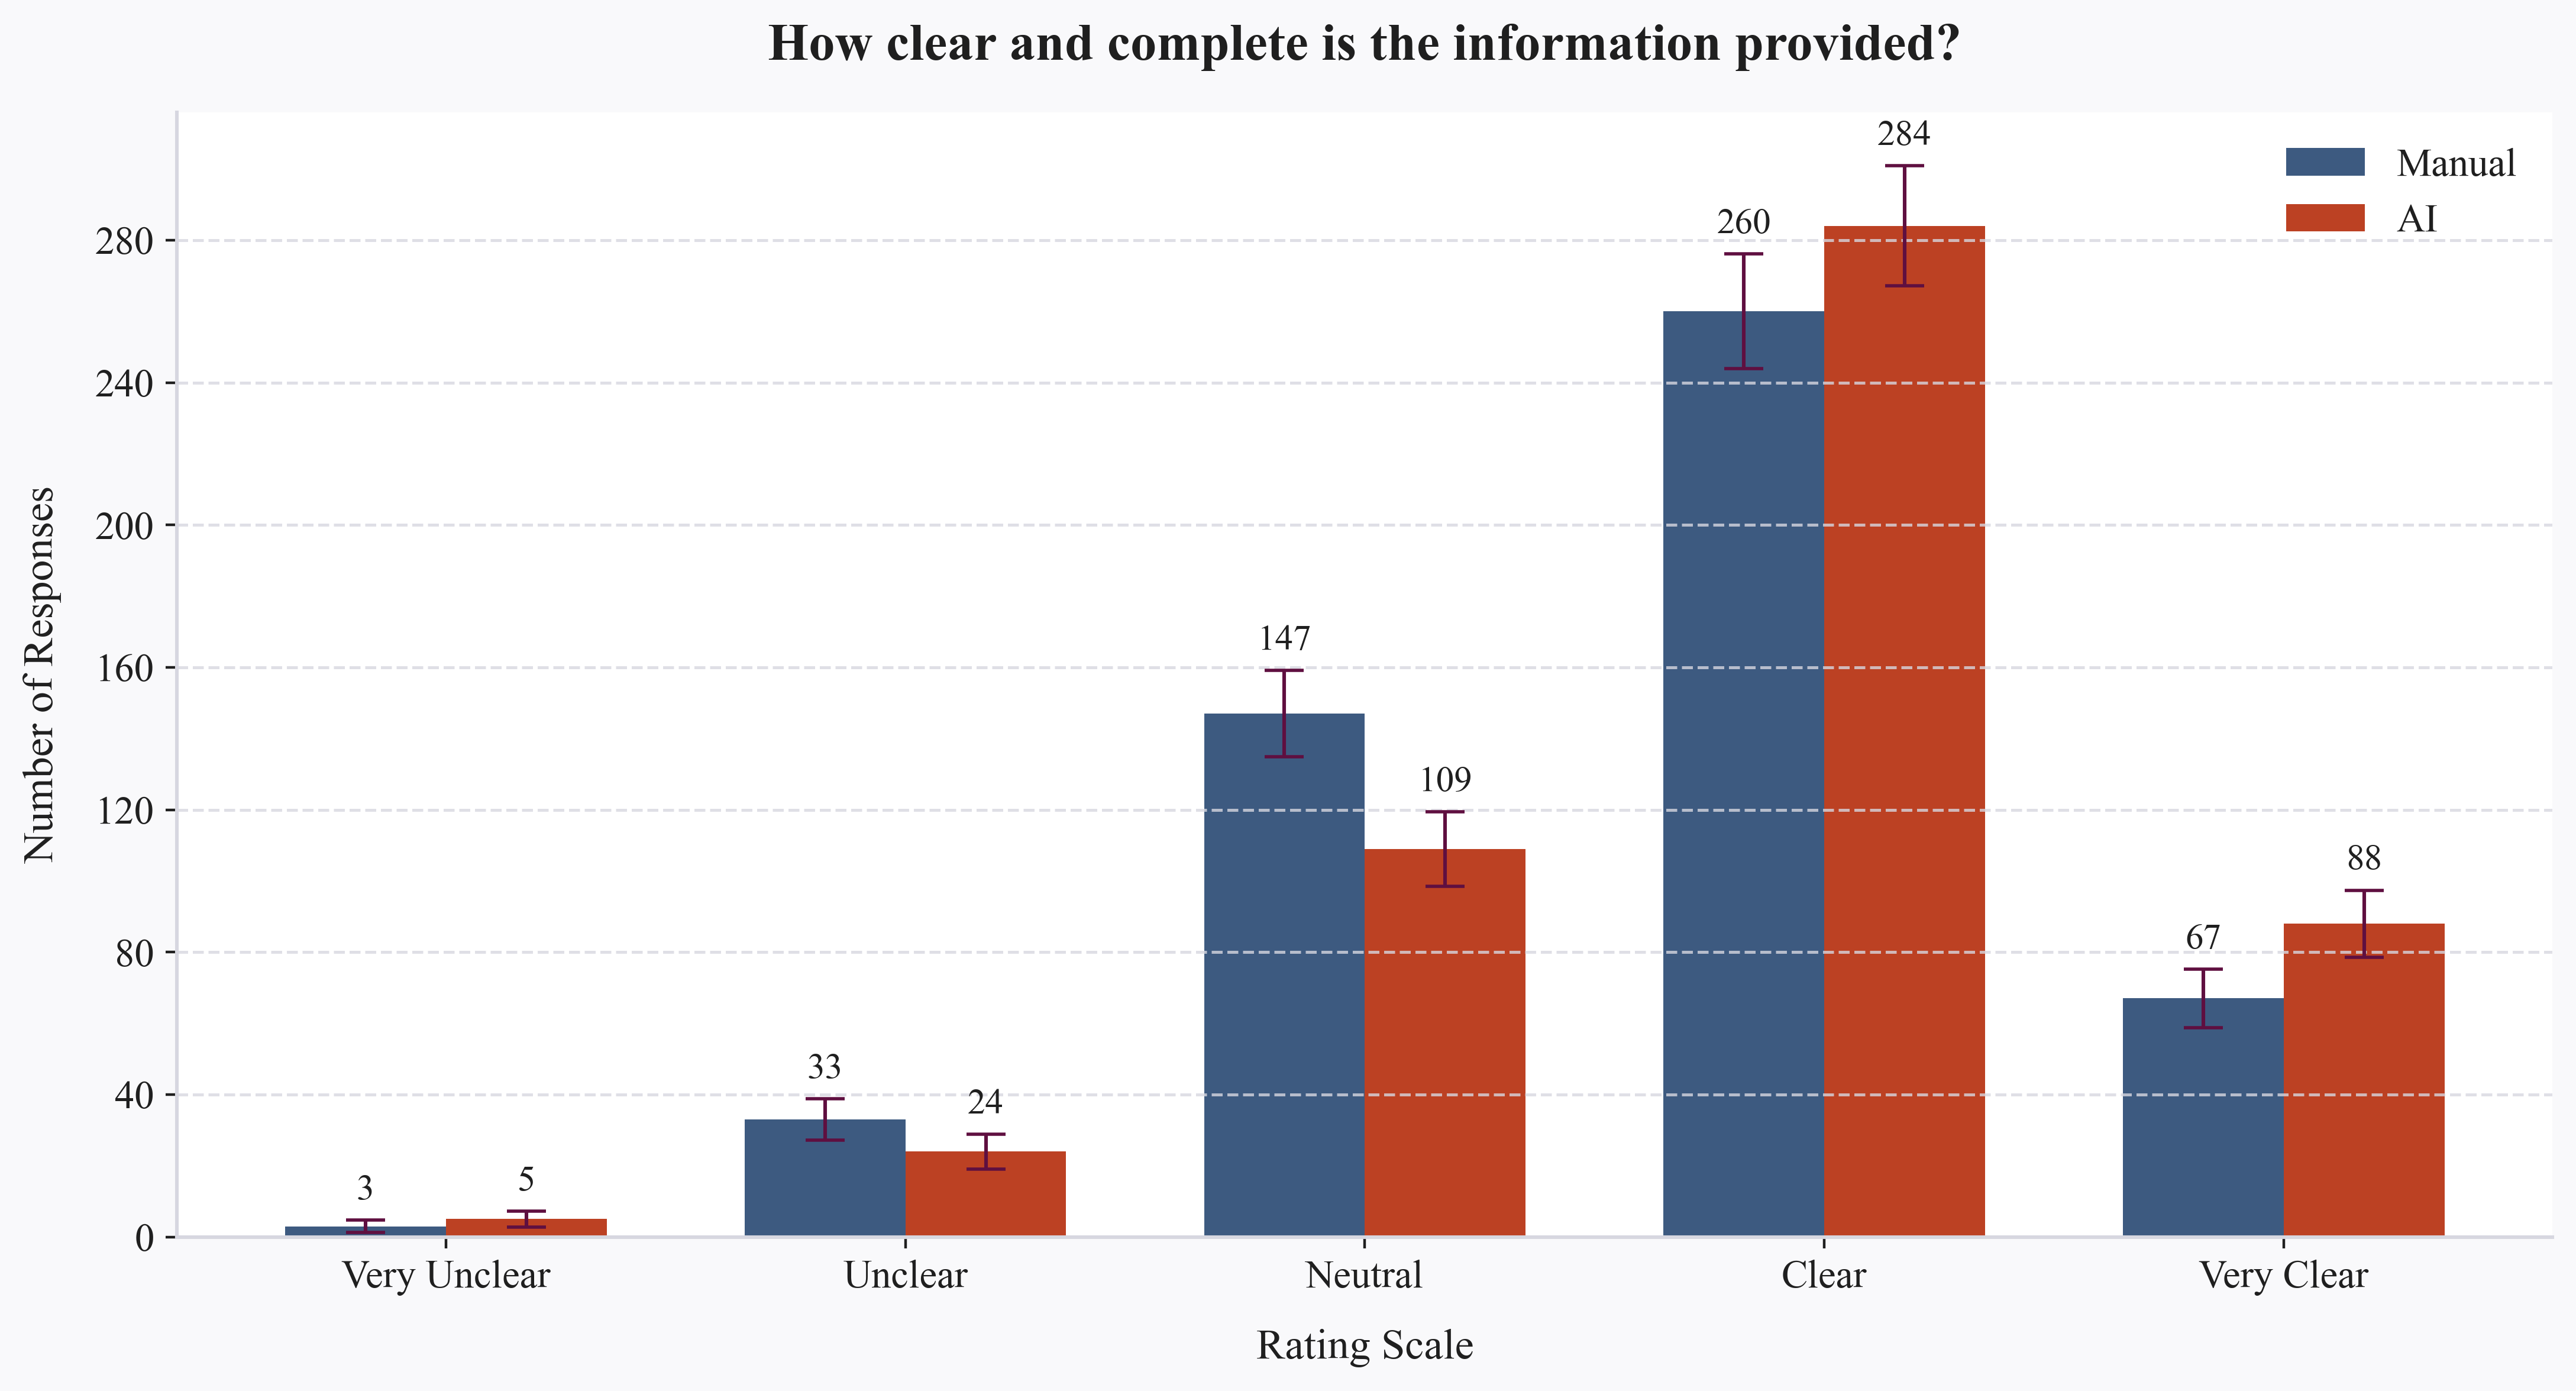
\includegraphics[width=0.85\linewidth]{figures/clarity_comparison.png}
  \caption{Comparison of perceived clarity and completeness between manual and AI-generated descriptions. Error bars represent Poisson-style standard error estimates computed on raw counts ($\sqrt{n}$).}
  \Description{Bar chart comparing manual and AI description ratings for clarity and information completeness}
  \label{fig:clarity}
\end{figure}

AI-generated descriptions were rated as clearer overall, with a notable reduction in neutral responses (109 vs.
147) and more ratings in the top two categories (Clear or Very Clear: 372 vs.
327). The pooled chi-square test indicated a statistically significant difference in the distribution ($\chi^2(4) = 11.47$, $p = 0.0218$). The effect size was small (Cramer's $V = 0.106$, computed with $N=1020$ pooled observations), consistent with a modest but systematic shift in perceived clarity.

\subsection{Comparative Preferences}
Beyond individual ratings, participants completed several comparative preference questions. Due to space constraints, this short paper reports the engaging comparison. Responses were nearly evenly split between AI-generated (221; 43.3\%) and manual (220; 43.1\%) descriptions, with 69 selections (13.5\%) indicating both versions were equally engaging. This near-parity suggests that personalization increased perceived clarity without reducing engagement.

\subsection{Overall Study Feedback}
Following the POI evaluations, participants were invited to provide optional overall feedback. A subset of 17 participants completed this section, rating three dimensions using a 5-point scale (1 = Poor, 5 = Excellent). The overall experience with POI descriptions received a mean rating of 3.88 (SD = 0.70, Median = 4.0), indicating generally positive reception. Participants expressed moderate to strong support for the concept of automatically adapting POI descriptions based on user interests, with a mean rating of 3.75 (SD = 0.93, Median = 4.0). Comfort with reading AI-generated descriptions when planning visits to new places received the highest mean rating of 3.94 (SD = 0.83, Median = 4.0), suggesting participants were receptive to AI-generated travel content when it demonstrated quality and relevance. The relatively low standard deviations (all below 1.0) indicate consensus among participants without extreme polarization of opinions.

Across metrics, AI adaptation primarily reduced neutral ratings and increased positive categories. Given the repeated-measures structure of the data, pooled tests summarize distributional shifts.


\section{Discussion}
This study investigated whether LLM-generated personalization of POI descriptions could enhance user engagement and perceived information quality while maintaining trustworthiness and accuracy. Our findings demonstrate that AI-adapted descriptions successfully achieved these objectives across multiple evaluation dimensions, with particularly notable improvements in clarity and trustworthiness.

\subsection{Effectiveness of AI Personalization}
The results reveal that AI-generated adaptations consistently shifted participant responses from neutral positions toward positive endorsements. Across all three core metrics (significance, trustworthiness, and clarity), we observed a compression of the neutral category and expansion of the top-box ratings. This pattern suggests that personalized descriptions help users form more confident and favorable assessments of POI value. The statistical significance achieved for clarity ($p = 0.0218$) and marginal significance for trustworthiness ($p = 0.050$) provide empirical support for the effectiveness of LLM-based personalization in travel content.

The near-parity in engagement preferences (221 AI vs. 220 manual) is particularly encouraging. It indicates that AI personalization does not merely optimize for a single dimension at the expense of others but rather maintains overall engagement quality while adding customization benefits. This balanced performance is critical for practical deployment, as travel platforms must ensure that personalized content remains compelling across diverse user segments.

\subsection{Trust as a Critical Factor}
The improvement in perceived trustworthiness warrants special attention. Trust is fundamental to POI recommendations, as users must believe the information is accurate and reliable before making travel decisions. The 50\% reduction in Not at all trustworthy ratings and the substantial increase in Extremely trustworthy ratings suggest that personalization, when executed thoughtfully, can enhance rather than undermine credibility. This finding challenges potential concerns that AI-generated content might be perceived as less authentic or reliable than human-authored descriptions.

We hypothesize that this trust enhancement stems from the alignment between description content and user interests. When information resonates with a user's stated preferences and travel style, it may be perceived as more relevant and therefore more credible. Additionally, the LLM's ability to maintain factual consistency while adjusting emphasis and framing likely contributed to maintaining high trust levels.

\subsection{Clarity Through Personalization}
The statistically significant improvement in clarity represents one of the study's most compelling findings. By adapting content to match user interests and expertise levels, AI-generated descriptions appear to communicate information more effectively. This suggests that generic, one-size-fits-all descriptions may inadvertently obscure key information for certain user segments. Personalization addresses this limitation by surfacing the most relevant details for each individual.

For example, a museum description personalized for a history enthusiast might emphasize historical context and artifacts, while the same POI described for a family traveler might highlight interactive exhibits and educational programs. Both versions convey accurate information but differ in emphasis and framing, resulting in clearer communication of value propositions aligned with user motivations.

\subsection{Participant Demographics and Generalizability}
Our participant pool consisted primarily of young, educated individuals (mean age 30.94 years) with intermediate to experienced travel backgrounds. The predominance of students and engineers suggests comfort with technology and potentially higher receptiveness to AI-generated content. These demographic characteristics may have contributed to the positive reception of personalized descriptions and high comfort levels with AI-authored travel content (mean = 3.94).

However, this demographic concentration also limits generalizability. Older travelers, those less familiar with AI technologies, or individuals from different cultural backgrounds might exhibit different preferences and trust patterns. The strong representation of Indian and German participants provides some international diversity but does not capture the full spectrum of global travel audiences.

\subsection{Implications for Tourism Platforms}
These findings have practical implications for travel and tourism platforms seeking to enhance user engagement. The results suggest that LLM-based personalization can be deployed to adapt POI descriptions dynamically without sacrificing trust or perceived information quality. Platforms could collect user preferences during onboarding or infer them from browsing behavior, then use LLMs to generate tailored descriptions that highlight aspects most relevant to each user.

The high comfort level with AI-generated content (mean = 3.94) indicates that transparency about AI involvement may not be a barrier to adoption, particularly among tech-savvy user segments. However, platforms should consider how to communicate the personalization process to maintain trust and set appropriate expectations.

\subsection{Limitations}
Several limitations should be acknowledged. First, participants evaluated descriptions in a controlled study environment rather than during actual trip planning, which may not fully capture real-world decision-making contexts. Second, the study did not track whether personalized descriptions influenced actual visit intentions or behaviors beyond stated preferences. Third, the within-subjects design, while enabling direct comparisons, may have introduced demand characteristics or heightened attention to differences between versions. Fourth, the study did not examine potential negative effects of over-personalization, such as filter bubbles or reduced serendipitous discovery of POIs outside user-stated interests.


\section{Conclusion}
This study demonstrates that large language models can effectively personalize POI descriptions to enhance user engagement and perceived information quality. Through a controlled user study with 51 participants evaluating 510 paired comparisons across 10 diverse POIs, we found that AI-generated adaptations significantly improved perceived clarity ($p = 0.0218$) and showed marginal improvements in trustworthiness ($p = 0.050$) compared to original manual descriptions. AI-personalized descriptions shifted user responses from neutral assessments toward stronger positive endorsements across all evaluated dimensions, while maintaining engagement levels comparable to carefully crafted manual content.

The findings reveal three key insights. First, personalization helps users form more confident and favorable assessments of POI value by surfacing information aligned with their interests and travel styles. Second, thoughtfully executed AI personalization can enhance rather than undermine perceived trustworthiness, challenging concerns about credibility of generated content. Third, participants expressed high comfort with AI-generated travel content (mean = 3.94 on a 5-point scale), suggesting receptiveness to this technology in tourism contexts.

These results have practical implications for travel platforms seeking to scale personalized experiences. LLM-based description adaptation offers a path to deliver customized content without the resource constraints of manual authoring for diverse user segments. However, deployment should consider demographic differences in receptiveness to AI content and implement strategies to prevent over-personalization from limiting serendipitous discovery.

This research contributes to the growing understanding of AI-powered personalization in tourism by demonstrating that content adaptation, not just recommendation, plays a valuable role in enhancing user experience. As large language models continue to advance, their application to travel content personalization presents opportunities to make tourism information more accessible, relevant, and engaging for diverse global audiences.


%%
%% The acknowledgments section is defined using the "acks" environment
%% (and NOT an unnumbered section). This ensures the proper
%% identification of the section in the article metadata, and the
%% consistent spelling of the heading.
% Acknowledgments are omitted for anonymous review.

%%
%% The next two lines define the bibliography style to be used, and
%% the bibliography file.
\bibliographystyle{ACM-Reference-Format}
\bibliography{PoI_GenAI}


\end{document}
\endinput
%%
%% End of file `sample-sigconf-authordraft.tex'.
